\section{Aufbau der Applikation}
\label{sec:Aufbau der Applikation}

\subsection{Einleitung}
Zur Entwicklung des \tool{}s wird wegen den im Kapitel Analyse erläuterten Gründen die Programmiersprache Go eingesetzt. Go erlaubt zwar einen Objekt-Orientierten Stil des Programmieren \cite[:240]{golang_faq}, bietet aber im Vergleich zu typisch \acs{OOP} Sprachen wie Java oder C++ keine Klassen \& Typen Hierarchien.

Anstatt der Klasse als Struktur bietet Go sogenannte Packages an. Innerhalb eines Package können beliebig viele .go Files erstellt werden die dann den Source Code enthalten. Private Variablen und Funktionen sind innerhalb eines Package frei zugänglich, können aber ausserhalb des Package nicht aufgerufen werden.

\begin{lstlisting}[language=bash, caption=Package Struktur des \tool{}]                    
github.com/ipsecdigatool/ipsecdigatool/       
	.git/
	capture/ # Pakete von Netzwerkadapter capturen        
		capture.go
	config/ # Konfiguration erstellen, laden, aktualisieren
		config.go
	logging/ # Syslog Nachrichten absetzen
		logging.go
	mtu/ # MTU Discovery durchfuehren
		analyze.go
		capture.go
		send.go
	packetloss/ # Packet loss feststellen
		detect.go
		espmap.go
		lostfile.go
	main.go # Programmstart und Daemon Funktionalitaet
\end{lstlisting}

Die Packages \code{capture}, \code{config}, \code{logging} werden sowohl für die \acs{MTU} Discovery als auch für die Packet Loss Detection verwendet. Die Packages \code{mtu} und \code{packetloss} werden nur für die jeweiligen Funktionen gebraucht und sind unabhängig voneinander. Das \code{main.go} enthält allen Code der für den Programmstart sowie den Daemon Mode gebraucht wird.

\subsection{Namenskonvention}
Go unterscheidet öffentlichen und privaten Funktionen und Variablen durch die Grosse- oder Kleinschreibung des ersten Buchstaben eines Funktions- oder Variablennamen. Gross geschriebene Namen zeigen eine öffentliche Funktion oder Variable an, die dann auch ausserhalb des Package genutzt werden kann.
In der Go Usergroup ist ausserdem auch die Idee verbreitet das Variablen- und Funktionsnamen möglichst kurz und prägnant sein sollen. CamelCase Namen sollen nach Möglichkeit vermieden werden. Dies kommt wohl einerseits von der C-Ähnlichkeit hat aber andererseits auch einen praktischen Grund. So ist ein Funktionsaufruf wie \code{capture.Start()} tatsächlich recht elegant und gut verständlich.
Im Verlauf dieses Projekts haben wir auch festgestellt dass es besser ist alle Namen, Ordnernamen und Kommandos wenn möglich klein zu schreiben. Zu Beginn des Projekts haben wir \code{github.com/IPsecDiagTool/IPsecDiagTool} als Repository Ordner Struktur verwendet und dies hat zu einigen Konflikten geführt. Glücklicherweise lassen sich Repositories auf github.com relativ leicht umbenennen und wir konnten auf eine rein klein geschriebene Ordner Struktur umsteigen.

\subsection{Programmstart & Multi-Threading}
Am Programmstart des \tool{} lässt sich das Zusammenspiel der verschiedenen Packages beobachten. Zuerst wird jeweils die Konfiguration geladen. Falls kein Konfigurationsfile auf dem System vorhanden ist wird ein neues File mit Default Werten erstellt. Danach werden die \code{logging} und \code{mtu} Packages initialisiert.

\begin{figure}[ht]
    \begin{center}
    % GFX Trim left bottom right top
        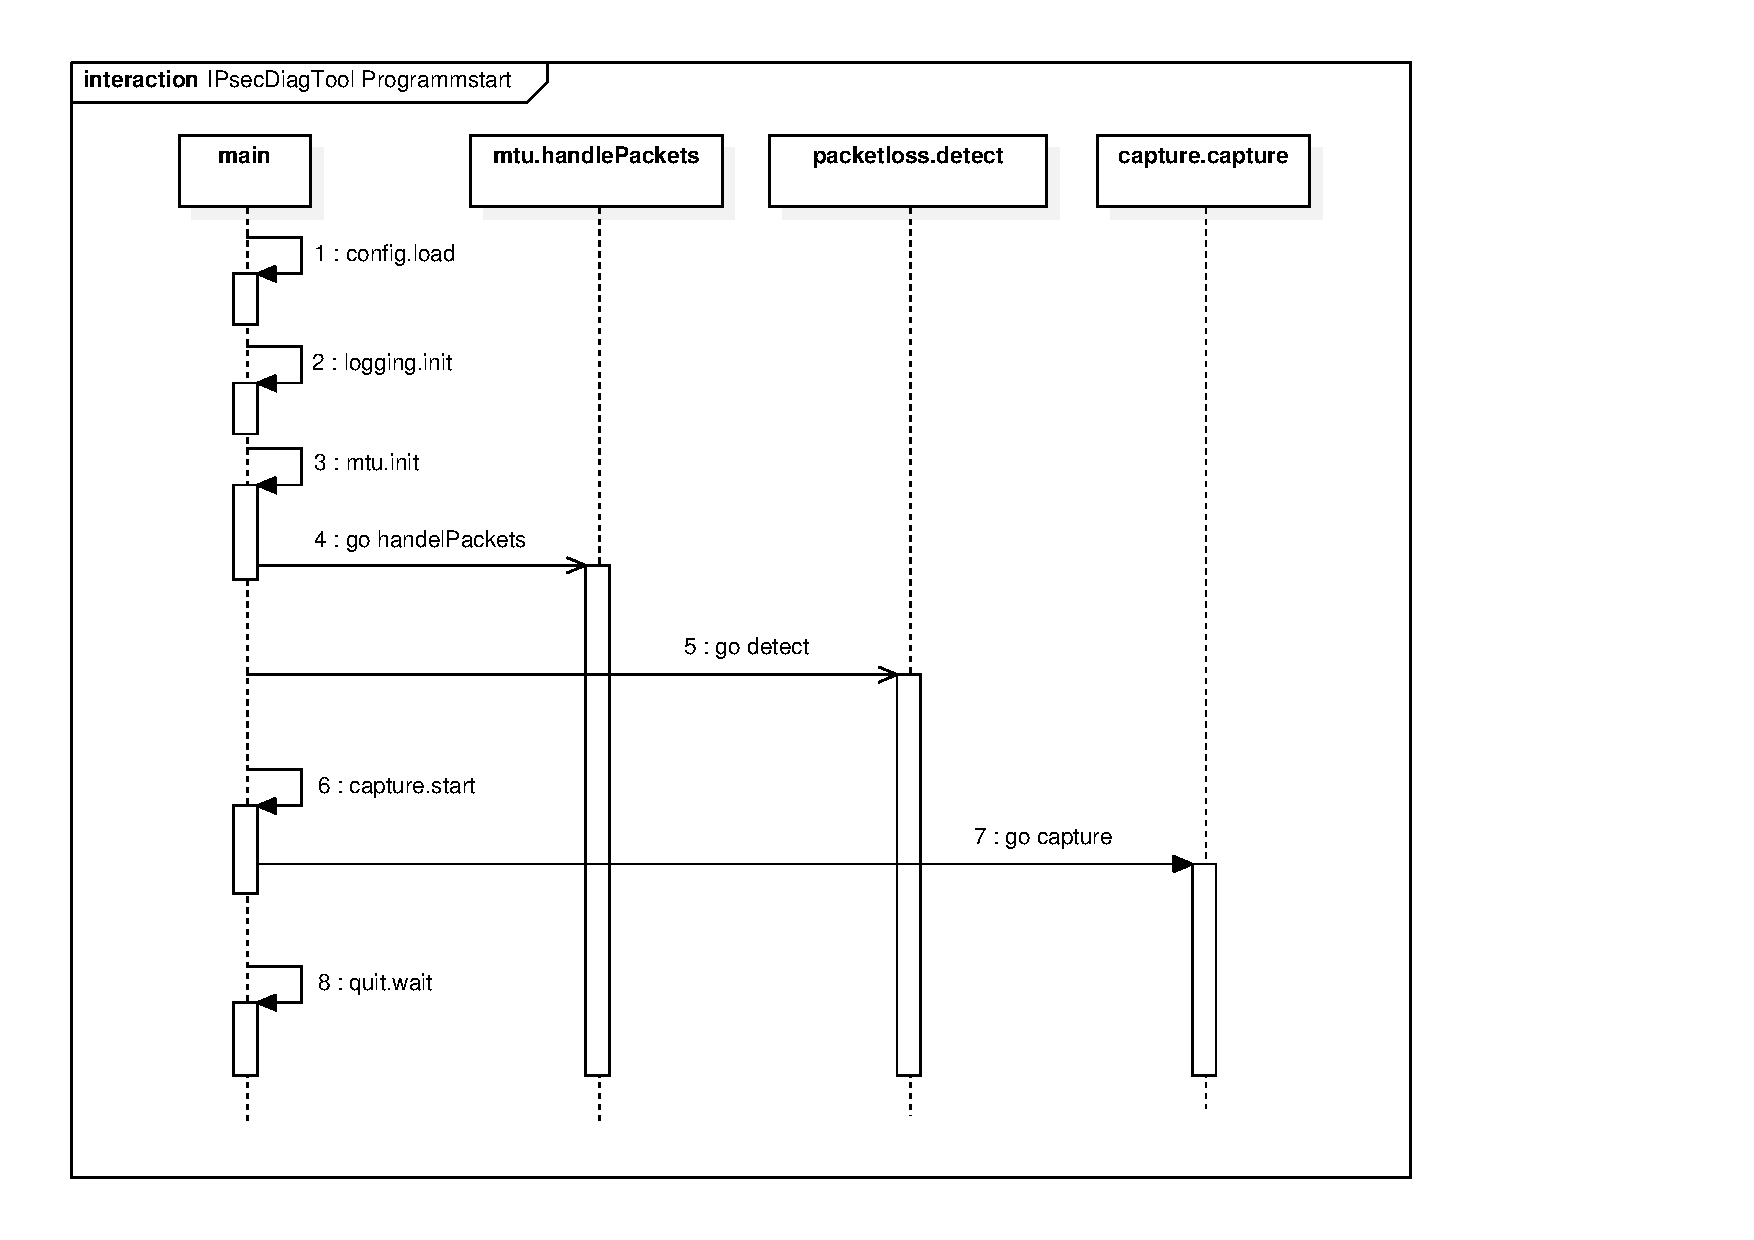
\includegraphics[trim=30 20 150 30,clip,width=\textwidth]{mainpart/implementation/img/programmstart}
    \end{center}
    \caption{Programmstart des \tool{}}
\end{figure}

Beim Initialiserungs-Vorgang der jeweiligen Package werden die fürs Multi-Threading notwendigen Konstrukte erstellt. Bei Go wird Multi-Threading vor allem via Goroutinen und Channels realisiert. Eine Goroutine ist eine Funktion die im gleichen Address Space, gleichzeitig mit anderen Goroutinen ausgeführt wird. Goroutinen sind leichtgewichtig und kosten bei der Erstellung nicht mehr als Stack Space. Um Nebenläufigkeit zu erreichen werden Goroutinen auf mehrere Threads des Betriebsystems multiplexed. When eine Goroutine blockiert, können die anderen Goroutinen weiterlaufen \cite[:1391]{effective_go}.
Zur Synchronisation und zum Datenaustausch zwischen Goroutinen werden sogenannte Channels verwendet. Typischerweise hat man in einer Goroutine eine for-Schleife und wartet darin auf Input aus einem Channel. Weitere, konkrete Beispiel werden im nächsten Abschnitt aufgezeigt.
\todo{Programmstart fertig machen.}


\todo{Abschnitt mit Goroutinen Code Beispielen.}


